\section{Parser Combinators for Path Querying}
\label{sec:combinators}

Parser combinators is a way to specify both a language syntax and a parser for it in terms of higher-order functions. 
Parser in this framework is a function which consumes a prefix of an input and returns either a parsing result or an error if the input is erroneous. 
Parser combinators compose parsers to form more complex parsers. 
A parser combinators library usually provides a set of a basic parser combinators, such as a combinator of the sequential application of the choice, but there can also be user-defined combinators.
Most parser combinators libraries, including the Meerkat library, can only process the linear input---strings or some kind of streams.
We modify the Meerkat library to work on the graph input.

%Parser combinators provide a way to specify a language syntax in terms of functions and operations on them. 
%A parser in this framework is usually a function which consumes a prefix of an input and returns either a parsing result or an error if the input is erroneous. 
%Parsers can be composed by using a set of parser combinators to form more complex parsers. 
%A parser combinators library provides with a set of basic combinators (such as sequential application or choice), and there can also be user-defined combinators. 
%Most parser combinators libraries, including the Meerkat library, can only process the linear input --- strings or some kind of streams. 
%We extend the Meerkat library to work on the graph input.

The following ideas are at the core of the modification.
%Extension is based on some common ideas.


\begin{itemize}
\item The intersection of a context-free and a regular language is context-free. There are several constructive proofs of this fact.
The proposed solution is a yet another constructive proof with the SPPF as a user-friendly representation of the context-free grammar for the intersection.
\item Linear input can be regarded as a linear directed graph with symbols of the input labeling the edges.
\item A conventional parser moves a pointer in the input from the position $i$ to the position $i+1$ and creates a new state when token between $i$-th and $i+1$-th positions matches what is required in the grammar.
In case of graph processing, there are possibly multiple ways to move from the current vertex $i$ and it is possible to produce multiple new states.
Generalized parsing is designed to optimally handle the production of multiple new states thus it is suitable to handle graph processing.
\item Matching a token in the input can be viewed as a predicate, for example $p_c (x) = x == c$. 
We can generalize this observation allowing matching of an edge label of an arbitrary type with a predicate of some sort.
\item If vertices of the graph contain any data of interest, we can treat them in the similar fashion as the edges. We can also convert the input graph transforming vertices into edges and then querying the transformed graph.
\end{itemize}


%\begin{itemize}
%\item Intersection of context-free language and regular one is a context-free language and there are different constructive proves of this fact.
%Proposed solution is a yet another constructive prove and SPPF is a just user-friendly representation of result context-free grammar.
%\item Linear input is a simple case of graph: positions are vertices and tokens are edges labels.
%Each edge is going from position (vertex) $i$ to position (vertex) $i+1$.
%\item Parser can move pointer in input from position $i$ to position $i+1$ and create new state when token between $i$ to position $i+1$ matches with required in grammar.
%In case of graph processing there are more then one ways to go from current vertex $i$ and it is possible to get more then one new state.
%Generalized parsing is designed to optimally handle steps which produce multiple new states and can handle help to handle this situation.
%\item We can treat the fact that token in input matches with required token from grammar as a predicate.
%This observation may be generalized: we can pass through  edge if its label satisfies some predicate.
%This way we can flexibly handle labels of arbitrary types.
%\item Vertex may be converted to edge: all incoming edges are convert to oncoming into source of new edge, all outgoing are convert to outgoing from target of new edge.
%This way we can handle vertex and edge labelled graphs as edge labelled.
%\end{itemize}

Querying process in our library is inherited from generalized parsing and is done in two steps.
The first step is ``parsing'': the construction of the SPPF which contains all derivation trees for the paths satisfying syntactic constraints.
The second step is semantic actions application which retrieves the necessary additional data about the paths from the SPPF.

\subsection{The Set of Combinators}

We demonstrate the set of combinators by example: the input graph, which represents a map, is presented in fig.~\ref{fig:graph}.
There are some cities connected by one-way roads represented by the edges labeled $road\_to$.
Each city is labeled by its name and a country it belongs to.

% \begin{figure}[h]
% 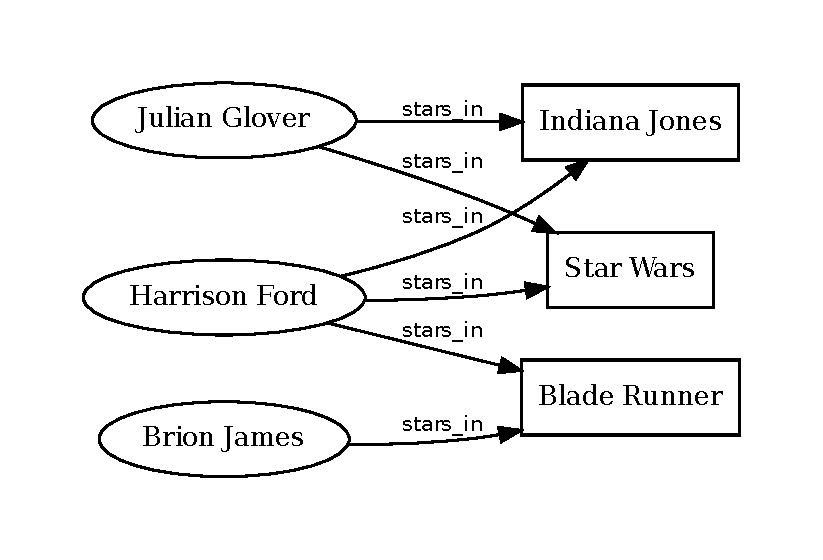
\includegraphics[width=0.45\textwidth]{graph}
% \caption{Example Input Graph of Roads}
% \label{fig:graph}
% \end{figure}

\begin{figure}[h]
\resizebox {0.45\textwidth} {!}
{
\begin{tikzpicture}[shorten >=1pt,node distance=2cm,on grid,auto] 
   \node[state] (a) [fill={rgb:black,1;white,2}]  {$a(X)$}; 
   \node[state] (b) [right=of a] {$b (Y)$}; 
   \node[state] (c) [right=of b] {$c (X)$}; 
   \node[state] (d) [left=of a] {$d (Y)$};
   \node[state] (e) [left=of d] {$e (X)$};
    \path[->] 
    (a) edge [bend left, above] node [above] {$road\_to$} (c)          
    (b) edge  node {$road\_to$} (a)
    (c) edge  node {$road\_to$} (b)
    (a) edge  node {$road\_to$} (d)
    (d) edge  node {$road\_to$} (e);
\end{tikzpicture}
}
\caption{Example graph. Vertex labels are in the form "city-name (country-name)"}
\label{fig:graph}
\end{figure}

Two basic building blocks of queries are the combinators for dealing with edges and vertices.
\begin{itemize}
    \item \lstinline{V[L](predicate: L =>   Boolean)} the combinator for processing vertices, where \lstinline{L} is a type of the node label. 
    Parsing with this combinator succeeds iff the vertex satisfies the predicate.
    \item \lstinline{E[N](predicate: N =>   Boolean)} the conbinator for processing edges, where \lstinline{N} is a type of the edge label. 
    Parsing with this combinator succeeds iff the edge satisfies the predicate.  
\end{itemize}

\begin{figure}[h]
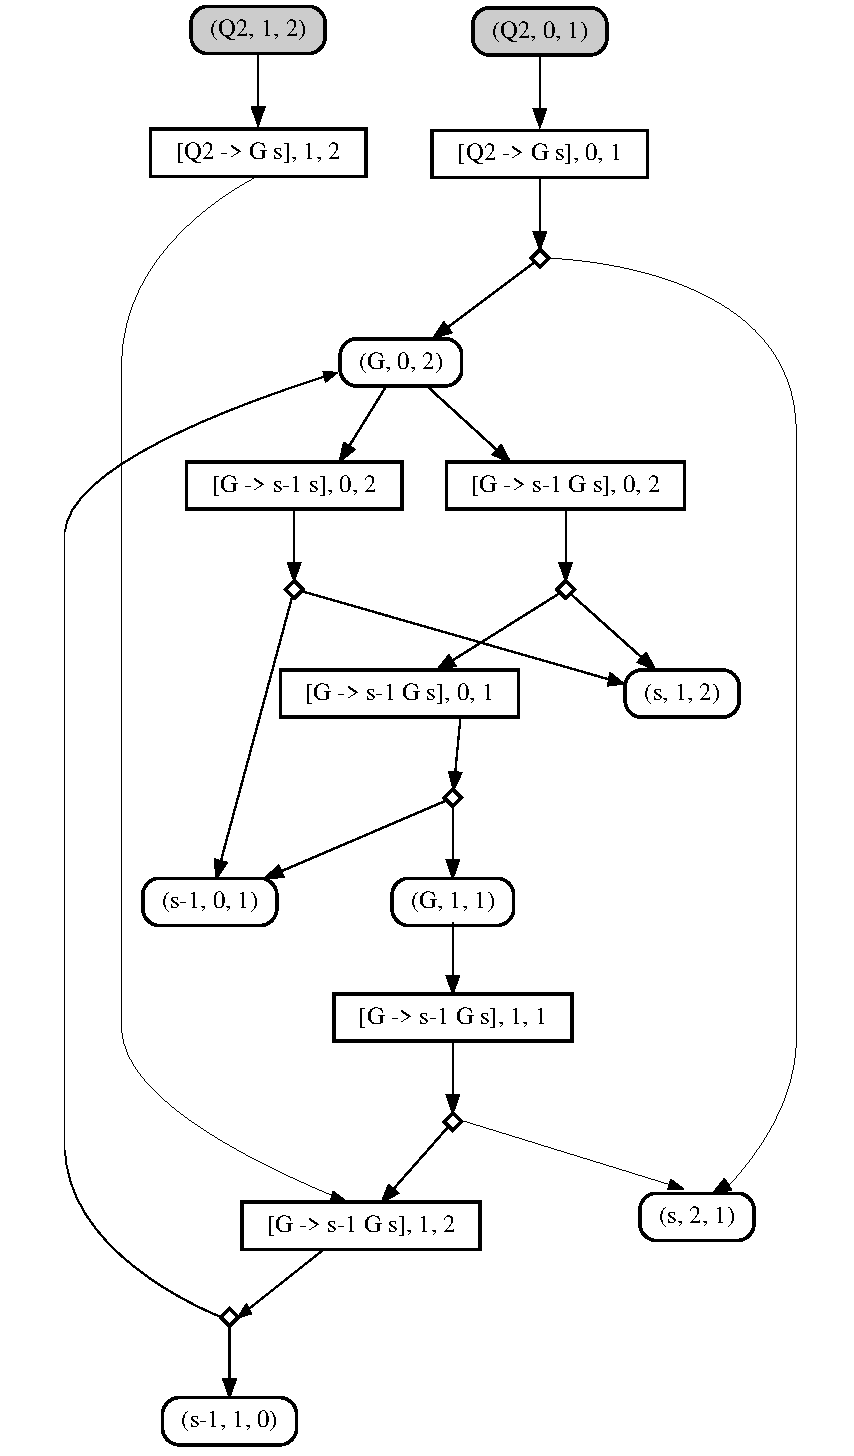
\includegraphics[width=0.49\textwidth]{sppf}
\caption{SPPF: result of applying cities query to the graph~\ref{fig:graph}}
\label{fig:sppf}
\end{figure}

To select cities which belong to some country, we can use the function \lstinline{V}: \lstinline{V[L]((e: Entity) =>   e.country =   "County Name")}.
Here \lstinline{Entity} is a property container for both edges and vertices. 
By using the \lstinline{Dynamic} trait, all accesses to properties (like \lstinline{(e: Entity).country}) are converted to the accesses to the properties of either a vertex or an edge.
For the sake of simplicity, we will omit \lstinline{Entity} type specifications for predicates. 
To query the graph for the paths from a city in the country $X$ to a city in the country $Y$, we need to sequentially compose the combinators for selecting the appropriate cities. 
A sequentialital combinator \lstinline{~} does just that: it sequentially  applies two queries one after the other. 
Let us denote a query for retrieving a city from the specific country \lstinline{city(name: String)} and a query for retrieving road edges \lstinline{roadTo}. 
With this denotation, a query \lstinline{city("X") ~ roadTo ~ city("Y")} returns the requested set of paths from the graph.
The complete query with all necessary subqueries is shown in fig.~\ref{fig:simpleQuery}.

\begin{figure}[h]
\begin{lstlisting}
def city(country: String) =
  V(_.country == country)
val roadTo = E(_.value() == "road_to")
val ourPath = 
  city("X") ~ roadTo ~ city("Y")
\end{lstlisting}
\caption{Path query}
\label{fig:simpleQuery}
\end{figure}

Having the query written, the next thing is to write a function to retrieve the actual data about the paths.
If we care only about the names of the cities, we can return a pair of the cities for each path.
First, we modify the query for vertices by adding the semantic action to it using the combinator \lstinline{^}: \lstinline{def city(name: String) =    syn(V(e.value() ==   name) ^ (_.value))}.
Then we need to actually map a path to a pair of cities: this is done with the combinator \lstinline{&}.
The complete query is in fig.~\ref{fig:simpleQueryV2}.
The result is the sequence of pairs of cities with the road between them.

%Now we would like to get all pair of cities which have a road between them. 
%So we need to transform our query to use semantic actions which is described in \ref{sec:semanticActions} section. 
%Now let us specify what we want from every our query. 
%From the \lstinline{city} query we want only city name, so we need to map a result of basic vertex combinator. 
%For that case we have a \lstinline{^} combinator we can write \lstinline{def city(name: String) = syn(V(e.value() == name) ^ (_.value))} to achieve  that. 
%In \lstinline{ourPath} query we need first and second cities to be represented as a pair. 
%For that we have a \lstinline{&} combinator which will map our sequence to a pair of strings.
%The final representation is shown on \ref{fig:simpleQueryV2}. 
%Now when we execute that query we will get a list which consists of all pairs of city's names which have a road between.

\begin{figure}[h]
\begin{lstlisting}
def city(country: String) =
  syn(V(_.country() == country) ^ (_.name))
val roadTo = E(_.value() == "road_to")
val ourPath = 
  syn(city("X") ~ roadTo ~ city("Y") &
    { case c0 ~ c1 => (c1, c2) })
\end{lstlisting}
\caption{Path query}
\label{fig:simpleQueryV2}
\end{figure}


The whole set of basic combinators, which our library provides, is presented in table~\ref{table:combinators}. 
There are two kind of combinators: the first kind combines parsers to form new parsers, meanwhile the second one is dedicated to the processing of the query result.
Whenever a string is used within a query, a parser which matches that string is implicitly generated.

\begin{table}[h]
\centering
\begin{tabular}{l@{}|l}
\multicolumn{1}{c|}{Combinator} & \multicolumn{1}{|c}{Description} \\ \hline
{\lstinline!a ~ b!} & sequential parsing: {\lstinline!a!} then {\lstinline!b!}   \\
{\lstinline!a | b!} & choice: {\lstinline!a!} or {\lstinline!b!}         \\
{\lstinline!a ?!}   & optional parsing: {\lstinline!a!} or nothing   \\
{\lstinline!a *!}   & repetition of zero or more {\lstinline!a!} \\
{\lstinline!a +!}   & repetition of at least one {\lstinline!a!} \\
{\lstinline!a ^ f!} & apply {\lstinline!f!} function to {\lstinline!a!} if  {\lstinline!a!} is a token \\
{\lstinline!a ^^!}  & capture output of {\lstinline!a!} if {\lstinline!a!} is a token    \\
{\lstinline!a & f!} & apply {\lstinline!f!} function to {\lstinline!a!} if  {\lstinline!a!} is a parser \\
{\lstinline!a &&!}  & capture output of {\lstinline!a!} if {\lstinline!a!} is a parser    \\
\hline
\end{tabular}
\caption{Meerkat combinators}
\label{table:combinators}
\end{table}


\subsection{Generic interface for input}
The combinators in our library are independent of the input representation. 
It is enough to specify two basic combinators which handle vertices and edges. 
Vertex handling is checking whether the vertex satisfies the given predicate.
In case of the edges, one needs to check which of the outgoing from the given vertex edges satisfy the given predicate. 
These two functions form the trait for the input (fig.~\ref{fig:input}).
It has two type parameters: the type of edge labels \lstinline{L} and the type of vertices labels \lstinline{N}.
We supported several different input sources:

%Combinators is a generic way to describe a query and when we have a query we want to execute that query on some graph considering it as an input for our query.
%The cool thing is that query execution mechanism may be fully separated from graph representation.
%We need only to have access to two very low-level functions, one for working with edges and one for vertices. 
%The first one would allow to get all edges outcoming from current vertex and also satisfies given predicate. 
%The second one will allow to check if current vertex satisfies given predicate.
%That interface is presented on fig~.\ref{fig:input}.
%It has two type parameters: \lstinline{L} for edge labels and \lstinline{N} for nodes.
%We have implementation of that input for the next data sources: 

\begin{itemize}
    \item Neo4jInput --- input source for the graph database Neo4j;
    \item GraphxInput --- input source for the graph presented in memory using GraphX library;
    \item LinearInput --- input source for the linear input data such as the ordinary strings.
\end{itemize}

\begin{figure}[h]
\begin{lstlisting}
trait Input[+L, +N] {
  def filterEdges(nodeId: Int, 
      predicate: L => Boolean): Seq[(L, Int)]
  def checkNode(nodeId: Int, 
      predicate: N => Boolean): Option[N]
}

\end{lstlisting}
\caption{Generalized input interface}
\label{fig:input}
\end{figure}

Since the required functions are simple, we believe it is possible to support most storages of graph-structured data.
Note, there are two technical limitations which arise from our decision to use values of the type \lstinline{Int} as unique identifiers for vertices (the \lstinline{nodeId} parameter).
It is impossible to correctly query the input graph with more than \lstinline{MAX_INT} vertices. 
Also there should be a way to provide such unique identifiers. Most systems already use unique identifiers by default, in other cases this feature can be implemented by the user.

%As far as required functions is very simple, we hope that this interface can be implemented for arbitrary storage of graph-structured data.
%Note, that currently we use \lstinline{Int} as unique identifier for nodes (the \lstinline{nodeId} parameter).
%It may be a technical restriction by the next two reason.
%\begin{itemize}
%\item It is impossible to use our library for correct processing of graph with more then \lstinline{MAX_INT} nodes. 
%\item It is necessary to provide such identifiers. Many systems use unique identifiers by default, but in some cases it may be necessary to implement required functionality manually.
%\end{itemize}



\subsection{Semantic Actions}
\label{sec:semanticActions}

Every path, which the query produces, has a derivation tree stored in the SPPF. 
The derivation tree is a very reach structure which can be hard to understand. 
To retrieve the data actually useful for the user, the library provides a mechanism of semantic actions. 
It is a way to apply some function to a parsed token or a subsequence. 

%Each path query produces a parse result stored in SPPF.
%This representation is very rich but hard to use and understand.
%That is why our library provides a mechanism which allows you to extract and process any useful data stored in parse result.
%This mechanism is called semantic actions.
%In general, they give you an opportunity to apply any function to parsed token or sequence.
%Now, let's understand how actions can be used in queries and how they are implemented in our library.

Semantic action binder for the tokens---vertices and edges alike---is \lstinline{^}. The most common use for it is to extract properties from the token and combine them in some fashion. 

%There are two main semantic action binders \lstinline{^} and \lstinline{&}.
%First of them is used when we need to perform some action on primitive tokens such as vertices or edges.
\begin{lstlisting}
// Defined in Terminal[+L] (edge) parser
def ^[U](f: L => U) = 
  new SymbolWithAction[L, Nothing, U] {...
  
// Defined in Vertex[+N] parser
def ^[U](f: N => U) = 
  new SymbolWithAction[Nothing, N, U] {...
\end{lstlisting}

For the combination of parsers there is a \lstinline{&} binder. Being  applied to a sequence of tokens, it can collect and process the data returned by the terminal parsers.
%Second is used when we need to process a result of combination of parsers.
\begin{lstlisting}
// Defined in Symbol[+L, +N, +V] parser
def &[U](f: V => U) = 
  new SymbolWithAction[L, N, U] {...
\end{lstlisting}

They both produce a new parser that parses the input exactly like the given parser but also have a bound function.
The function is referenced in each SPPF node produced by the corresponding parser.

%But actually, they both have the same behaviour, they produce a new parser that has the same parsing possibilities as an original parser but also have a binded function.
%Then, every SPPF node that will be produced by parser with binded function will have a reference to this function too.

%These binders along with the other combinators 

%So, these operations in composition with other combinators provides an instrument for data processing on which most queries are based. 
%For example, \lstinline{^} can extract some data from tokens and \lstinline{&} applied to sequence of tokens can collect and process data returned by terminal parsers.

The way semantic actions are executed has mostly remained the same as in the original Meerkat library: semantic actions are first executed for the children of the current node, then the results are collected and passed to a semantic action of the current node. 
If there are ambiguous nodes in the SPPF, the original Meerkat library just throws an exception. 
In our case, ambiguity can arise not only when there are multiple derivations of a string but ambiguous nodes can also represent several different subpaths which are derived from the respective nonterminal.
We chose to provide a way to extract the derivation trees from the SPPF lazily, since the number of the paths can be infinite. 
Unambiguous trees are yielded with a breadth-first search.


%The main idea of execution of semantic actions remained the same as in the original Meerkat library excepting one aspect.
%For each node we still just execute all actions of its children, collect results and pass them as argument to current function.
%But what should executor do if SPPF has ambiguous nodes? 
%Previous implementation just throws an exception in that case and it is reasonable because original library is written for linear parsing and most grammars allows disambiguation in that case.

%However, even unambiguous grammar can produce ambiguous derivations during parsing of graphs.
%That's why we provide a feature that makes it possible to extract ``all'' trees stored in SPPF.
%The number of path deriving from given grammar can be infinite, for example, when graph has cycles.
%This reason we can provide only a lazy stream of trees that allows to take as much of them as you need.
%Our solution is based on breadth first search that yields an unambiguous SPPF corresponding to some derivation immediately after it was found.

The composition of the extraction of trees and the semantic action execution is called \lstinline{executeQuery}.
It parses the input graph from all positions, produces a list of SPPF roots, extracts all derivations from every root, executes semantic actions and returns a lazy stream of results.